\documentclass[10pt,a4paper]{article}
\usepackage[margin=15mm,top=12mm,bottom=14mm]{geometry}
\usepackage[T1]{fontenc}
\usepackage{lmodern,amsmath,graphicx,booktabs,fancyvrb,xcolor,siunitx,array}
\sisetup{group-minimum-digits=4}
\usepackage[hidelinks]{hyperref}
\usepackage{titlesec}
\titlespacing*{\section}{0pt}{8pt}{3pt}
\titlespacing*{\subsection}{0pt}{6pt}{2pt}
\pagestyle{plain}
\setlength{\parindent}{0pt}
\setlength{\parskip}{3pt}
\begin{document}
\noindent{\Large\textbf{Weisshorn nose cone at 720 mm: geometry for SolidWorks}}\\[2pt]
2027\_C\_FD\_NOSE-CONE-720MM\_GEOMETRY \hfill Fabio Feig (FD), 30.10.2026
\par\medskip\hrule\medskip

\section*{Design A: LV-Haack, 3U payload inside the nose (baseline)}
LV-Haack profile, $679.0 + 41 = 720.0$\,mm. $x$ along
the axis from the blunted tip, $r$ the outer radius, mm.

\centerline{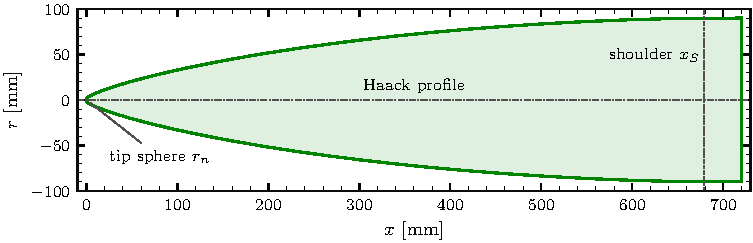
\includegraphics[width=0.92\linewidth]{figures/profile_A.pdf}}
\vspace{-6pt}
\begin{align*}
\text{Spherical tip}\quad & 0 \le x \le x_T: & r &= \sqrt{r_n^2-(r_n-x)^2}\\
\text{Haack profile}\quad & x_T \le x \le x_S: & r &= \frac{R}{\sqrt{\pi}}\sqrt{\theta-\frac{\sin 2\theta}{2}+C\sin^3\theta},\qquad
x=\frac{L}{2}\,(1-\cos\theta)-\delta,\quad \theta_T \le \theta \le \pi\\
\text{Coupler cylinder}\quad & x_S \le x \le x_S + c: & r &= R
\end{align*}

\begin{minipage}[t]{0.44\linewidth}\vspace{0pt}\small
\begin{tabular}{@{}ll@{}}
\toprule
Parameter & Value\\
\midrule
Haack constant $C$ & $1/3$\\
Length to the sharp apex $L$ & 682.345\\
Body radius $R$ & 90.000 ($D = 180$)\\
Tip radius $r_n$ & 4.500\\
Length removed by the tip $\delta$ & 3.345\\
Tangency point $(x_T, r_T)$ & (2.434, 3.998)\\
Tangency angle $\theta_T$ [rad] & 0.1843209\\
Shoulder $x_S$ & 679.000\\
Coupler cylinder $c$ & 41.000\\
\textbf{Total length} & \textbf{720.000}\\
\bottomrule
\end{tabular}

\smallskip
Tangent to the sphere at $x_T$ and to the cylinder at $x_S$ ($\mathrm{d}r/\mathrm{d}x = 0$).
\end{minipage}\hfill
\begin{minipage}[t]{0.53\linewidth}\vspace{0pt}\scriptsize
\begin{tabular}{@{}rr|rr|rr@{}}
\toprule
$x$ & $r$ & $x$ & $r$ & $x$ & $r$\\
\midrule
0.000 & 0.000 & 250.000 & 59.269 & 525.000 & 85.042 \\
2.434 & 3.998 & 275.000 & 62.625 & 550.000 & 86.307 \\
25.000 & 13.022 & 300.000 & 65.750 & 575.000 & 87.404 \\
50.000 & 20.651 & 325.000 & 68.657 & 600.000 & 88.333 \\
75.000 & 27.183 & 350.000 & 71.356 & 625.000 & 89.087 \\
100.000 & 33.006 & 375.000 & 73.857 & 650.000 & 89.652 \\
125.000 & 38.295 & 400.000 & 76.167 & 675.000 & 89.983 \\
150.000 & 43.149 & 425.000 & 78.293 & 679.000 & 90.000 \\
175.000 & 47.635 & 450.000 & 80.239 & 700.000 & 90.000 \\
200.000 & 51.796 & 475.000 & 82.010 & 720.000 & 90.000 \\
225.000 & 55.666 & 500.000 & 83.610 &  &  \\
\bottomrule
\end{tabular}
\end{minipage}

\subsection*{SolidWorks}
Sketch on the Front Plane, origin at the blunted tip, $x$ (rocket axis) to the right, document units mm.
\begin{enumerate}\setlength{\itemsep}{1pt}
\item \textbf{Tip:} Centerpoint Arc, centre $(4.500,\,0)$, from $(0,\,0)$ to $(x_T,\,r_T) = (2.434,\,3.998)$.
\item \textbf{Haack profile:} Tools $\rightarrow$ Sketch Entities $\rightarrow$ Equation Driven Curve $\rightarrow$
  \emph{Parametric}; paste (angles in radians, $t$ is $\theta$):
\begin{Verbatim}[frame=single,fontsize=\small,xleftmargin=0pt]
x_t = 341.172513*(1 - cos(t)) - 3.345026
y_t = 50.777063*sqr(t - sin(2*t)/2 + 0.3333333*sin(t)^3)
t1  = 0.1843209
t2  = pi
\end{Verbatim}
  The curve starts on the arc end $(x_T, r_T)$ and ends at $(x_S,\,R) = (679.000,\,90.000)$;
  add a Tangent relation between the arc and the curve.
\item \textbf{Coupler:} Line from $(679.000,\,90.000)$ to $(720.000,\,90.000)$,
  then a line down to the axis and a centreline along the axis from the tip.
\item \textbf{Solid:} Revolved Boss, 360$^\circ$ about the centreline (outer mould line; shell and joint by ST).
\end{enumerate}
CAD: \texttt{nose\_lvhaack\_L682\_c41\_rn4.5mm.step} (solid).

\newpage

\section*{Design B: Von K\'arm\'an, 3U payload not in the nose (backup)}
Von K\'arm\'an profile, $700.0 + 20 = 720.0$\,mm. $x$ along
the axis from the blunted tip, $r$ the outer radius, mm.

\centerline{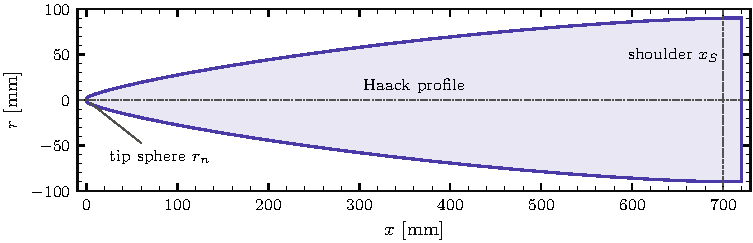
\includegraphics[width=0.92\linewidth]{figures/profile_B.pdf}}
\vspace{-6pt}
\begin{align*}
\text{Spherical tip}\quad & 0 \le x \le x_T: & r &= \sqrt{r_n^2-(r_n-x)^2}\\
\text{Haack profile}\quad & x_T \le x \le x_S: & r &= \frac{R}{\sqrt{\pi}}\sqrt{\theta-\frac{\sin 2\theta}{2}+C\sin^3\theta},\qquad
x=\frac{L}{2}\,(1-\cos\theta)-\delta,\quad \theta_T \le \theta \le \pi\\
\text{Coupler cylinder}\quad & x_S \le x \le x_S + c: & r &= R
\end{align*}

\begin{minipage}[t]{0.44\linewidth}\vspace{0pt}\small
\begin{tabular}{@{}ll@{}}
\toprule
Parameter & Value\\
\midrule
Haack constant $C$ & $0$\\
Length to the sharp apex $L$ & 705.465\\
Body radius $R$ & 90.000 ($D = 180$)\\
Tip radius $r_n$ & 4.500\\
Length removed by the tip $\delta$ & 5.465\\
Tangency point $(x_T, r_T)$ & (2.916, 4.212)\\
Tangency angle $\theta_T$ [rad] & 0.2184214\\
Shoulder $x_S$ & 700.000\\
Coupler cylinder $c$ & 20.000\\
\textbf{Total length} & \textbf{720.000}\\
\bottomrule
\end{tabular}

\smallskip
Tangent to the sphere at $x_T$ and to the cylinder at $x_S$ ($\mathrm{d}r/\mathrm{d}x = 0$).
\end{minipage}\hfill
\begin{minipage}[t]{0.53\linewidth}\vspace{0pt}\scriptsize
\begin{tabular}{@{}rr|rr|rr@{}}
\toprule
$x$ & $r$ & $x$ & $r$ & $x$ & $r$\\
\midrule
0.000 & 0.000 & 250.000 & 51.442 & 525.000 & 80.831 \\
2.916 & 4.212 & 275.000 & 54.781 & 550.000 & 82.712 \\
25.000 & 11.036 & 300.000 & 57.975 & 575.000 & 84.444 \\
50.000 & 17.201 & 325.000 & 61.030 & 600.000 & 86.013 \\
75.000 & 22.609 & 350.000 & 63.953 & 625.000 & 87.400 \\
100.000 & 27.535 & 375.000 & 66.746 & 650.000 & 88.578 \\
125.000 & 32.106 & 400.000 & 69.412 & 675.000 & 89.494 \\
150.000 & 36.393 & 425.000 & 71.952 & 700.000 & 90.000 \\
175.000 & 40.443 & 450.000 & 74.366 & 720.000 & 90.000 \\
200.000 & 44.287 & 475.000 & 76.653 &  &  \\
225.000 & 47.948 & 500.000 & 78.809 &  &  \\
\bottomrule
\end{tabular}
\end{minipage}

\subsection*{SolidWorks}
Sketch on the Front Plane, origin at the blunted tip, $x$ (rocket axis) to the right, document units mm.
\begin{enumerate}\setlength{\itemsep}{1pt}
\item \textbf{Tip:} Centerpoint Arc, centre $(4.500,\,0)$, from $(0,\,0)$ to $(x_T,\,r_T) = (2.916,\,4.212)$.
\item \textbf{Haack profile:} Tools $\rightarrow$ Sketch Entities $\rightarrow$ Equation Driven Curve $\rightarrow$
  \emph{Parametric}; paste (angles in radians, $t$ is $\theta$):
\begin{Verbatim}[frame=single,fontsize=\small,xleftmargin=0pt]
x_t = 352.732280*(1 - cos(t)) - 5.464559
y_t = 50.777063*sqr(t - sin(2*t)/2)
t1  = 0.2184214
t2  = pi
\end{Verbatim}
  The curve starts on the arc end $(x_T, r_T)$ and ends at $(x_S,\,R) = (700.000,\,90.000)$;
  add a Tangent relation between the arc and the curve.
\item \textbf{Coupler:} Line from $(700.000,\,90.000)$ to $(720.000,\,90.000)$,
  then a line down to the axis and a centreline along the axis from the tip.
\item \textbf{Solid:} Revolved Boss, 360$^\circ$ about the centreline (outer mould line; shell and joint by ST).
\end{enumerate}
CAD: \texttt{nose\_vonkarman\_L705\_c20\_rn4.5mm.step} (solid).

\end{document}
